\documentclass[12pt, a4paper]{article}
\usepackage[utf8]{inputenc}
\usepackage{amsmath}
\usepackage{amsthm}
\usepackage{amssymb}
\usepackage{graphicx}
\usepackage{parskip}
\usepackage{hyperref}
\usepackage{fancyhdr}
\usepackage{lastpage}
\usepackage[vlined,ruled]{algorithm2e}
\usepackage[acronym]{glossaries}
\usepackage{caption}
\usepackage{titlesec}
\usepackage{tikz}
\usetikzlibrary{arrows,automata}

\titleformat{\section}
  {\normalfont\bfseries}{Problem 9.\thesection}
  {0em}{}

\titleformat{\subsection}
  {\normalfont\bfseries}{9.\thesubsection}
  {0em}{}

\titleformat{\subsubsection}
  {\normalfont\bfseries}{9.\thesubsection}
  {0em}{}

\title{%
  Stochastic Network Modeling \\
  Homework 9 - Solutions
}
\author{%
  Juan Pablo Royo Sales\\
  \small{Universitat Politècnica de Catalunya}
}
\date\today

\pagestyle{fancy}
\fancyhf{}
\fancyhead[C]{}
\fancyhead[R]{Juan Pablo Royo Sales - UPC MIRI}
\fancyhead[L]{SNM - Homework 9}
\fancyfoot[L,C]{}
\fancyfoot[R]{Page \thepage{} of \pageref{LastPage}}
\setlength{\headheight}{15pt}
\renewcommand{\headrulewidth}{0.4pt}
\renewcommand{\footrulewidth}{0.4pt}

\renewcommand{\qedsymbol}{$\blacksquare$}

\begin{document}

\maketitle

\section{}
\subsection{}
It should fullfil that $p_{ij} = p_{ji}^r$ or filling the Komologov criteria.

\subsection{}
If the chain is reversible it must fullfil the following equality

\begin{subequations}
  \begin{align}
    p_{12}p_{23}p_{31} &= p_{13}p_{32}p_{21}\\
    \frac{2}{12}\frac{3}{6}\frac{1}{2} &= \frac{3}{12}\frac{1}{2}\frac{2}{6}\\
  \end{align}
\end{subequations}
It is reversible. Then doing the equations for calculating the stationary distribution we get:

\begin{subequations}
  \begin{align}
    \begin{cases}
      \pi_{0} &= \frac{1}{G}\\
      \pi_{1} &= \frac{1}{G} \frac{6}{7}\\
      \pi_{2} &= \frac{1}{G} \frac{6}{7} \frac{1}{2}\\
      \pi_{3} &= \frac{1}{G} \frac{6}{7} \frac{1}{2}\\
    \end{cases}
  \end{align}
\end{subequations}

Therefore,

\begin{subequations}
  \begin{align}
      G &= 1 + \frac{6}{7} + \frac{6}{7} \frac{1}{2} + \frac{6}{7} \frac{1}{2}\\
        &= \frac{19}{7}
  \end{align}
\end{subequations}

Therefore, 
\begin{subequations}
  \begin{align}
    \begin{cases}
      \pi_0 &= \frac{7}{19}\\
      \pi_1 &= \frac{6}{19}\\
      \pi_2 &= \frac{3}{19}\\
      \pi_3 &= \frac{3}{19}\\
    \end{cases}
  \end{align}
\end{subequations}

\subsection{}
\begin{subequations}
  \begin{align}
    \begin{cases}
      \pi_1\frac{7}{12} &= \pi_0\frac{1}{2}\\
      \pi_1\frac{2}{12} &= \pi_2\frac{2}{6}\\
      \pi_1\frac{3}{12} &= \pi_3\frac{1}{2}\\
      \sum pi_i = 1
    \end{cases}
  \end{align}
\end{subequations}

\subsection{}
\begin{subequations}
  \begin{align}
      \pi_1\frac{7}{6} &= \pi_0\\
      \pi_1\frac{1}{2} &= \pi_2\\
      \pi_1\frac{1}{2} &= \pi_3\\
      \pi_1 &= \frac{1}{1 + \frac{7}{6} + \frac{1}{2} + \frac{1}{2}}\\
            &= \frac{6}{19}
  \end{align}
\end{subequations}

Therefore, 
\begin{subequations}
  \begin{align}
    \begin{cases}
      \pi_0 &= \frac{7}{19}\\
      \pi_1 &= \frac{6}{19}\\
      \pi_2 &= \frac{3}{19}\\
      \pi_3 &= \frac{3}{19}\\
    \end{cases}
  \end{align}
\end{subequations}

\subsection{}
\begin{subequations}
  \begin{align}
    \begin{cases}
      \pi_{1} &= \frac{1}{G} \\
      \pi_{2} &= \frac{1}{G} \frac{1}{2}\\
      \pi_{3} &= \frac{1}{G} \frac{1}{2}\\
    \end{cases}
  \end{align}
\end{subequations}

\begin{subequations}
  \begin{align}
      G &= 1 + \frac{1}{2} + \frac{1}{2}\\
        &= 2
  \end{align}
\end{subequations}

Therefore, 
\begin{subequations}
  \begin{align}
    \begin{cases}
      \pi_1 &= \frac{1}{2}\\
      \pi_2 &= \frac{1}{4}\\
      \pi_3 &= \frac{1}{4}\\
    \end{cases}
  \end{align}
\end{subequations}

\section{}
\subsection{}
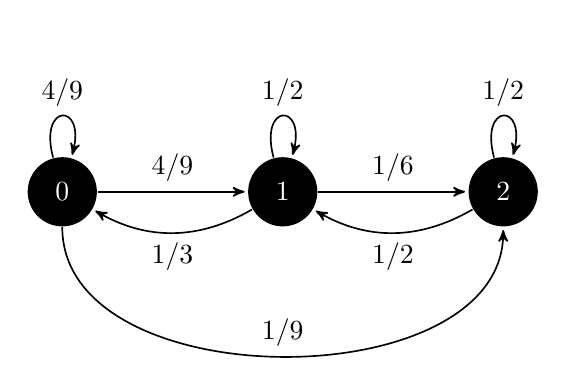
\begin{tikzpicture}[->,>=stealth',shorten >=1pt,auto,node distance=2.8cm,
  semithick]
  \tikzstyle{every state}=[fill=black,draw=none,text=white]

  \node[state]         (A)              {0};
  \node[state]         (B) [right of=A] {1};
  \node[state]         (C) [right of=B] {2};

  \path (A) edge              node {4/9} (B)
        (A) edge [loop above] node {4/9} (A)
        (B) edge [bend left]  node {1/3} (A)
        (B) edge              node {1/6} (C)
        (B) edge [loop above] node {1/2} (B)
        (C) edge [bend left]  node {1/2} (B)
        (C) edge [loop above] node {1/2} (C)
        (A) edge [bend right=90] node {1/9} (C)
        ;
\end{tikzpicture}
\begin{align*}
  P = \begin{bmatrix}
       & 0 & 1 & 2\\
     0 & 4/9 & 4/9 & 1/9\\
     1 & 1/3 & 1/2 & 1/6 \\
     2 & 0 & 1/2 & 1/2 \\
\end{bmatrix}
\end{align*}

\subsection{}
Tree is reversible because it forms a tree

\subsection{}
$I_{dl} = (\pi_0 + \pi_1)r = (\frac{9}{31}+\frac{15}{31})\frac{1}{2} = \frac{12}{31}$

\subsection{}
$L = (\pi_1 + \pi_2)s = (\frac{15}{31}+\frac{7}{31})\frac{1}{2} = \frac{11}{31}$

\subsection{}
\begin{subequations}
  \begin{align}
    E[N] &= \sum_{i=0}^\infty (ps)^{n-1}r\\
         &= \sum_{i=0}^\infty \frac{1}{6}^{n-1}\frac{1}{2}\\
         &= \frac{1}{2}\frac{1}{(1-\frac{1}{6})^2}\\
         &= \frac{18}{25}
  \end{align}
\end{subequations}

\end{document}

